\documentclass[12pt]{article}
\usepackage[top=1in, bottom=1in, left=1.5in, right=1in]{geometry}
\usepackage{float}
\usepackage{graphicx}
\usepackage{listings}
\usepackage{fullpage}
\usepackage{color}
\usepackage{graphicx}
\usepackage{hyperref}
\usepackage{caption}
\usepackage{subcaption}
\graphicspath{ ./ }
\renewcommand{\baselinestretch}{1.5}

\definecolor{codegreen}{rgb}{0,0.6,0}
\definecolor{codegray}{rgb}{0.5,0.5,0.5}
\definecolor{codepurple}{rgb}{0.58,0,0.82}
\definecolor{backcolour}{rgb}{0.95,0.95,0.92}

\lstset{
    backgroundcolor=\color{backcolour},
    commentstyle=\color{codegreen},
    keywordstyle=\color{magenta},
    numberstyle=\tiny\color{codegray},
    stringstyle=\color{codepurple},
    basicstyle=\tiny,
    breakatwhitespace=false,
    breaklines=true,
    captionpos=b,
    keepspaces=true,
    numbers=left,
    columns=fixed,
    basewidth=.5em,
    numbersep=5pt,
    showspaces=false,
    showstringspaces=false,
    showtabs=false,
    tabsize=2
}

\hypersetup{
    colorlinks,
    citecolor=black,
    filecolor=black,
    linkcolor=black,
    urlcolor=black
}

\begin{document}

\begin{titlepage}

\begin{center}

\renewcommand{\baselinestretch}{1.5}
\Large \textbf { A BASIC, FOUR LOGIC CLUSTER, DISJOINT SWITCH CONNECTED FPGA ARCHITECTURE }\\[0.8in]

\normalsize
\textbf{ A SENIOR PROJECT REPORT}\\[0.1in]
 \small
       \textit{\textbf{Submitted in partial fulfillment of
        the requirements for the award of the degree of}}\\[0.3in]
\normalsize
       \textbf{ BACHELOR OF SCIENCE \\IN\\ COMPUTER ENGINEERING}\\[0.5in]

% Submitted by
 by \\
\textbf{ JOSEPH PRACHAR }

\vspace{.3in}
Under the guidance of\\
{\textbf{ Dr. Tina Smilkstein }}\\[0.1in]

\vfill

% Bottom of the page

\includegraphics[height=1.8in]{logo}\\[0.1in]
{Department of Computer Engineering}\\
\normalsize
\textsc{ California Polytechnic State University, San Luis Obispo }\\
March 2018\\
\textcolor{red}{\textbf{VERSION 0.4}}


\end{center}

\end{titlepage}

\begin{abstract}
This paper seeks to describe the process of developing a new FPGA architecture from 
nothing, both in terms of knowledge about FPGAs and in initial design material. Specifically,
 this project set out to design an FPGA architecture which could implement a simple 
state machine type design with less than 10 inputs, less than 10 outputs and less 
than 10 states. The open source Verilog-to-Routing FPGA CAD flow tool was used in order to
synthesize, place, and route HDL files onto the architecture. The hardware implementation of this project was completed
making use of the cadence suite of software tools (mainly Gennus, Innovus, and Virtuoso)
and Global Foundries CMRF8SF 130nm process.
This project was completed in terms of the original goals and proved to be limited by
the general place and route algorithm, when a much more specific algorithm should have been
used for such a routing constrained architecture.

\end{abstract}
\newpage

\tableofcontents
\newpage
\listoffigures
\newpage
\lstlistoflistings
\newpage

\section{Introduction}

\subsection{Overview}

FPGA’s are some of the most complicated digital circuits on the market today. They 
can help companies build a custom digital circuit with years less development time 
compared to an ASIC design process. This project aims to be an exploratory exercise
into the implementation details of the FPGA through the creation 
of a basic FPGA architecture. This new architecture will be extremely simple in nature 
due to the vastly intricate circuit that needs to be created and the complex software 
required to route designs within it.

This project will focus on pulling together the many basic overviews provided by 
the research sources listed in the bibliography <cite unused articles here>. The main technical overview that will 
be used to guide the development of this new architecture is Muhammad Imran Masud’s
master's thesis (FPGA Routing Structures: A Novel Switch Block and Depopulated 
Interconnect Matrix Architectures) \cite{masud_1999}. Masud provides a wealth of general overview details 
of both switch block and interconnect matrix designs before presenting his own variations 
on them. As the target of this project is just to develop a basic working FPGA design,
the focus will be on using the general overview of these complicated blocks rather 
than Masud’s experimental versions to increase simplicity of the design.

While this project will not create any ripples in the electrical and computer engineering 
field, it will be an extremely useful exercise in digital circuit design, verification,
and tool production. Designing the new architecture is only a slice of the overall 
time requirement of this project. A large amount of time must also be spent verifying 
this design, which will provide much practice with simulation/verification software 
due to the complicated nature of this circuit. The individual blocks of this circuit 
should be straightforward to test, but when performing system level testing, a design 
must first be created and loaded into the fpga which presents an interesting challenge.
This challenge leads into the last part of this project, tool development. As this 
is a completely new FPGA architecture, completely new place, route, and bitstream generation tools must 
be created in order to implement designs and actually use this project. Fortunately,
early on in the development of this project, the open source Verilog-to-Routing \cite{vtr} CAD flow
tool was discovered. This mean that the exceptionally complicated place and route component
of this project did not need to be created from scratch. Together, the three separate
components of this project (design, test, and software tools) come together to provide an
excersise encompassing a large breadth of the computing field.

\subsection{Basic Logic Element}

The most fundamental of all parts of an FPGA architecture is the basic logic element 
(BLE). The BLE is the component which actually does the computation in the circuit.
BLE’s are made up of a combination of look-up tables and flip flops. Given enough 
of these BLE’s, any digital circuit can be created; this provides the 
basic foundation for the FPGA’s circuit emulation capabilities.

\begin{figure}[ht]
\centering
\begin{subfigure}{.5\textwidth}
    \centering
    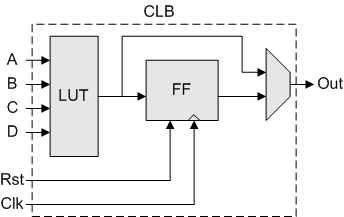
\includegraphics[width=.95\textwidth]{simple_ble}
    \caption{Simple BLE design (Figure from \cite{simple_ble})}
    \label{fig:simple_ble}
\end{subfigure}%
\begin{subfigure}{.5\textwidth}
  \centering
  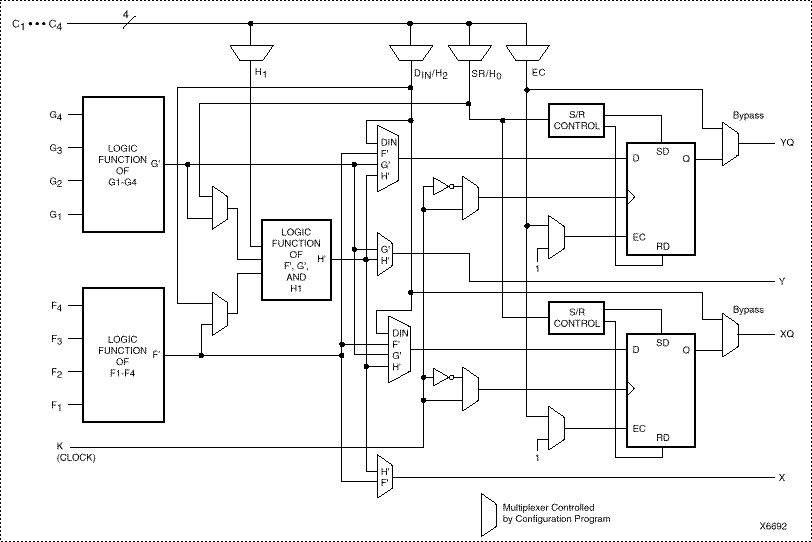
\includegraphics[width=.95\textwidth]{complex_ble}
  \caption{Xilinx XC4000 BLE design (Figure from \cite{xilinx_xc4000})}
  \label{fig:complex_ble}
\end{subfigure}
\caption{Comparison of BLE design}
\label{fig:compare_ble}
\end{figure}

There are many variable factors that determine the form and function of a BLE in 
any given architecture (as can be seen in Figure \ref{fig:compare_ble}): Number of inputs to the block, number of LUT’s, size of each 
LUT, and number of flip-flops to name a few. As a general rule, the more complicated 
the BLE, the less signals need to be routed by the global interconnect. This makes 
logical sense seeing as when a circuit is broken into more sub-circuits (as needed 
with a few input BLE) there are more nets connecting BLE’s together. This increases 
the minimum bus width of the interconnect fabric in order to achieve the same route-ability 
as an architecture featuring a more complicated BLE design.

In opposition, a large BLE design with many LUTs and flip flops may reduce congestion 
on the interconnect fabric but makes the architecture more prone to inefficient use 
of its logic resources, since there may be a significant unused portion of each LUT 
in each complicated BLE. Ultimately, the most efficient BLE design is dependant on 
the use case for the final hardware, with general purpose FPGA’s often using a combination 
of 2 4-LUT’s paired with a smaller 3-LUT and 2 flip flops, as in the Xilinx XC4000EX 
architecture (Figure \ref{fig:complex_ble}) \cite{xilinx_xc4000}. This allows the
routing software to use this BLE as 2 separate 4-LUT 
BLE’s or one larger 5-LUT BLE, thereby partially circumventing the inefficiency problem. 

\subsection{Connection Box}\label{Conn_Box}

\begin{figure}[ht]
  \centering
  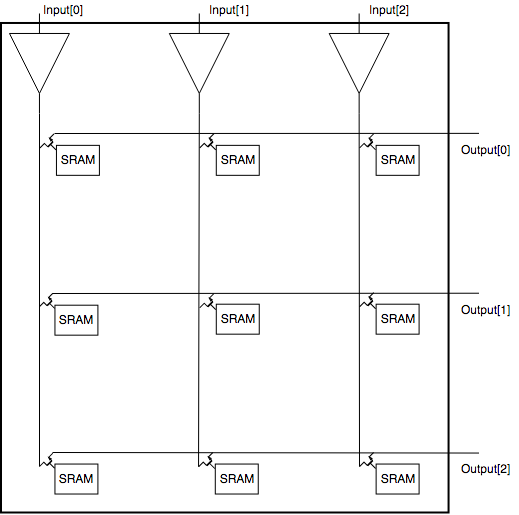
\includegraphics[width=.5\textwidth]{conn_box}
  \caption{3 input 3 output connection box}
  \label{fig:conn_box}
\end{figure}

The Connection Box (CB) is a unidirectional switching block allowing signals 
to enter and exit the general fabric bus of the FPGA. A simple (fully-connected) CB design 
would consist of each output pin from the module being connected to a mux which could 
select from any of the inputs (or none of them). Another of way to implement this module would be to 
have two buses of wires running perpendicular to each other on different layers of 
silicon. These two buses would be connected at each ‘crossing’ with a transistor 
which can short the circuit between the two different bus domains as can be seen in
Figure \ref{fig:conn_box}. Both of these simple Connection Box designs allow any of
the input pins to be directed to any number of the output pins.


\subsection{Logic Cluster} \label{logicCluster}

\begin{figure}[ht]
  \centering
  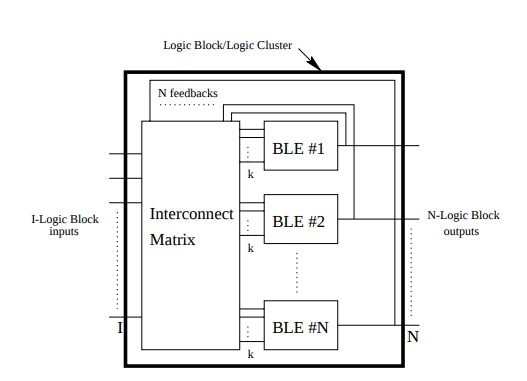
\includegraphics[width=.7\textwidth]{logicclusterex}
  \caption{General logic cluster diagram (Figure from \cite{masud_1999})}
  \label{fig:logiccluster_ex}
\end{figure}

A strategy to put less stress on the fabric of the FPGA while also retaining a simple 
BLE design is to use the concept of a Logic Cluster to introduce a separation in 
global routing resources and local routing resources. A Logic Cluster is simply a 
group of BLE’s combined with a connection box (now referred to as an interconnect matrix)
so that a more complex operation 
can be performed without being routed through the general interconnect. Usually, 
there are 4 to 16 BLE’s per Logic Cluster which all have their outputs connected 
as inputs into the main interconnect matrix as well as out of the module (into the 
general interconnect). This enables other BLE’s in the same logic cluster to use 
those outputs, enabling more complicated designs to be created without using global 
routing resources at all (for the intermediate signals).

\subsection{Switch Block}
The switch block is fundamentally just as important as the BLE is to the basic FPGA 
architecture. Combinations of this block create the entire FPGA routing scheme and 
allow signals to be dynamically routed throughout the design so that any digital 
circuit can be implemented. A switch block is generally designed as a bidirectional 
switch that acts as the interchange for the intersection of 4 buses of the FPGA fabric.
There are also unidirectional switch blocks, although these designs require larger 
bus widths to achieve the same route-ability in exchange for the simpler switch design.

\begin{figure}[ht]
  \centering
  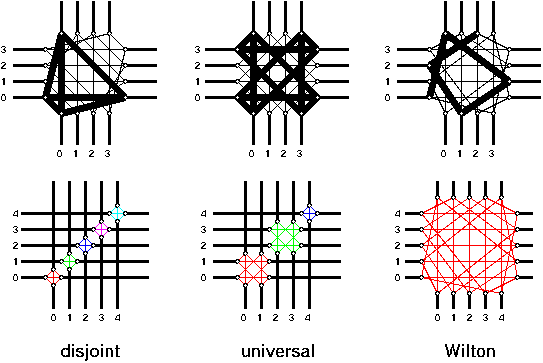
\includegraphics[width=.6\textwidth]{switch_blocks}
  \caption{Comparison of connection patterns of modern switch blocks (Figure from \cite{switch_blocks})}
  \label{fig:switch_blocks}
\end{figure}

There are many different strategies to determine which bus wires are able to be connected 
to each other as seen in Figure \ref{fig:switch_blocks}. The simplest of these is the disjoint
connection pattern. As the name 
suggests, this strategy creates separate routing domains from each wire in each bus 
and once a signal is in one domain it is not able to be routed through any other 
domain. For example, if 4 10-bit buses are using a disjoint switch block as an interchange,
the first wire in the top bus can only be connected to the first wire in the other 
3 buses, not any of the other wires. This does decrease route-ability due to having 
separate domains but is also a very predictable and easily understandable strategy.
Other strategies (such as the wilson or universal patterns) create several orders 
of magnitudes greater number of possible routes to get from point to point and thus 
require much more complicated routing algorithms.

\subsection{Input/Output Block}

\begin{figure}[ht]
    \centering
    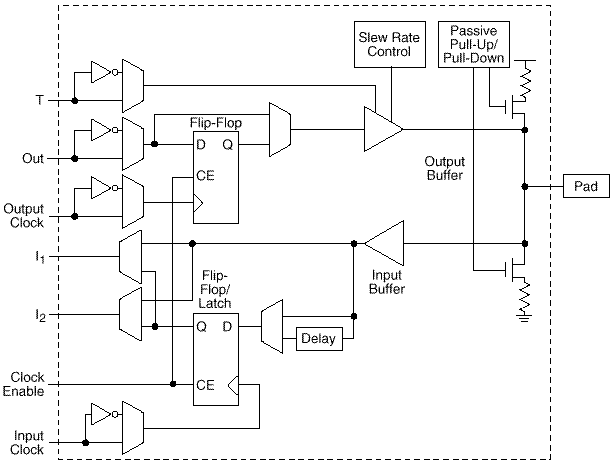
\includegraphics[width=0.75\textwidth]{complex_io}
    \caption{Xilinx XC4000 IO block (Figure from \cite{xilinx_xc4000})}
    \label{fig:complex_io}
\end{figure}

The IO block is another of the essential components of an FPGA, although its function
is notably simpler than any of the other blocks previously discussed. The IO block's
purpose is as simple as it sounds, provide a configurable way for signals to get onto and off of
the chip. As is a reoccurring theme in FPGA design, this is a fairly simple block to
grasp yet there are very complex implementations of them on modern commercial FPGA's
as can be seen with the XC4000's IO block (Figure \ref{fig:complex_io}). This example of
a fully featured IO block contains both input and output flip-flops, output slew rate
control, pull down/pull up resistors, and configurable output voltage levels. This
however, is not necessary as the simplest implementation is simply 2 transmission gates
and 2 buffers which allow the isolation and selection of the input/output lines from
the pad.

\subsection{Architecture} \label{Architecture}

\begin{figure}[ht]
    \centering
    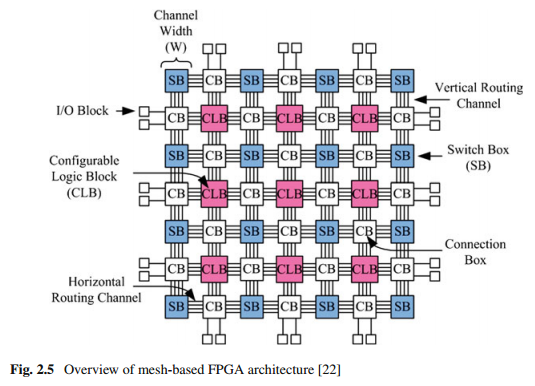
\includegraphics[width=0.75\textwidth]{generalarch}
    \caption{General island-style FPGA architecture (Figure from \cite{fpga_arch_overview})}
    \label{fig:island_style}
\end{figure}

When all of these types of previously discussed blocks are put together into a complete
design, the result looks something like the architecture in Figure \ref{fig:island_style}.
The logic clusters (which
feature the computational elements and are labeled CLB for configurable logic block in this
 diagram) act as the 'islands' while the general interconnect
resides in the channels in between. At each crossing of vertical and horizontal fabric
buses a switch block is placed to allow the connection of different bus wires. This is
the most popular style of FPGA currently in use today due to its vast amount of routing
resources and repetitive design elements.


\newpage
\section{Design Overview}

This new FPGA architecture, at a high level, will consist of three types of blocks:
IO, switch, and logic cluster. Each of these blocks will be completely configurable 'in circuit'
via the use of chained shift registers throughout the entire chip. Once again, due 
to the potential complexity of this circuit and the desire to complete this project,
only a basic working design is being targeted. This means that no one circuit design
metric will be targeted to be improved on from other existing FPGA architectures.
The rough scope/goals for the final circuit will be the ability to implement simple
finite state machine type circuits with less than 10 inputs, less than 10 outputs, and
less than 10 states. Although with the use of Verilog-to-Routing, any verilog design
which fits onto the architecture may be implemented.

This project consists of essentially three parts of equal time and value: circuit 
design, circuit validation, and implementation tools. This document contains many 
arbitrary design decisions. From research, it is clear what a generalized FPGA design 
looks like and how it is routed. What has become increasingly difficult is specifying 
the actual values of the device. Width of interconnect buses, interconnect redundancy,
and routing connectedness to IO blocks are all examples of things that are very 
much “hand waved” based on all available research. The following three 
sections represent a rough hashing out of such values. These were constantly 
re-evaluated throughout the design process to insure that each value provides a meaningful 
connection towards the final 10-input, 10-output, 10-state FSM implementation goal.

\begin{figure}[ht]
  \centering
  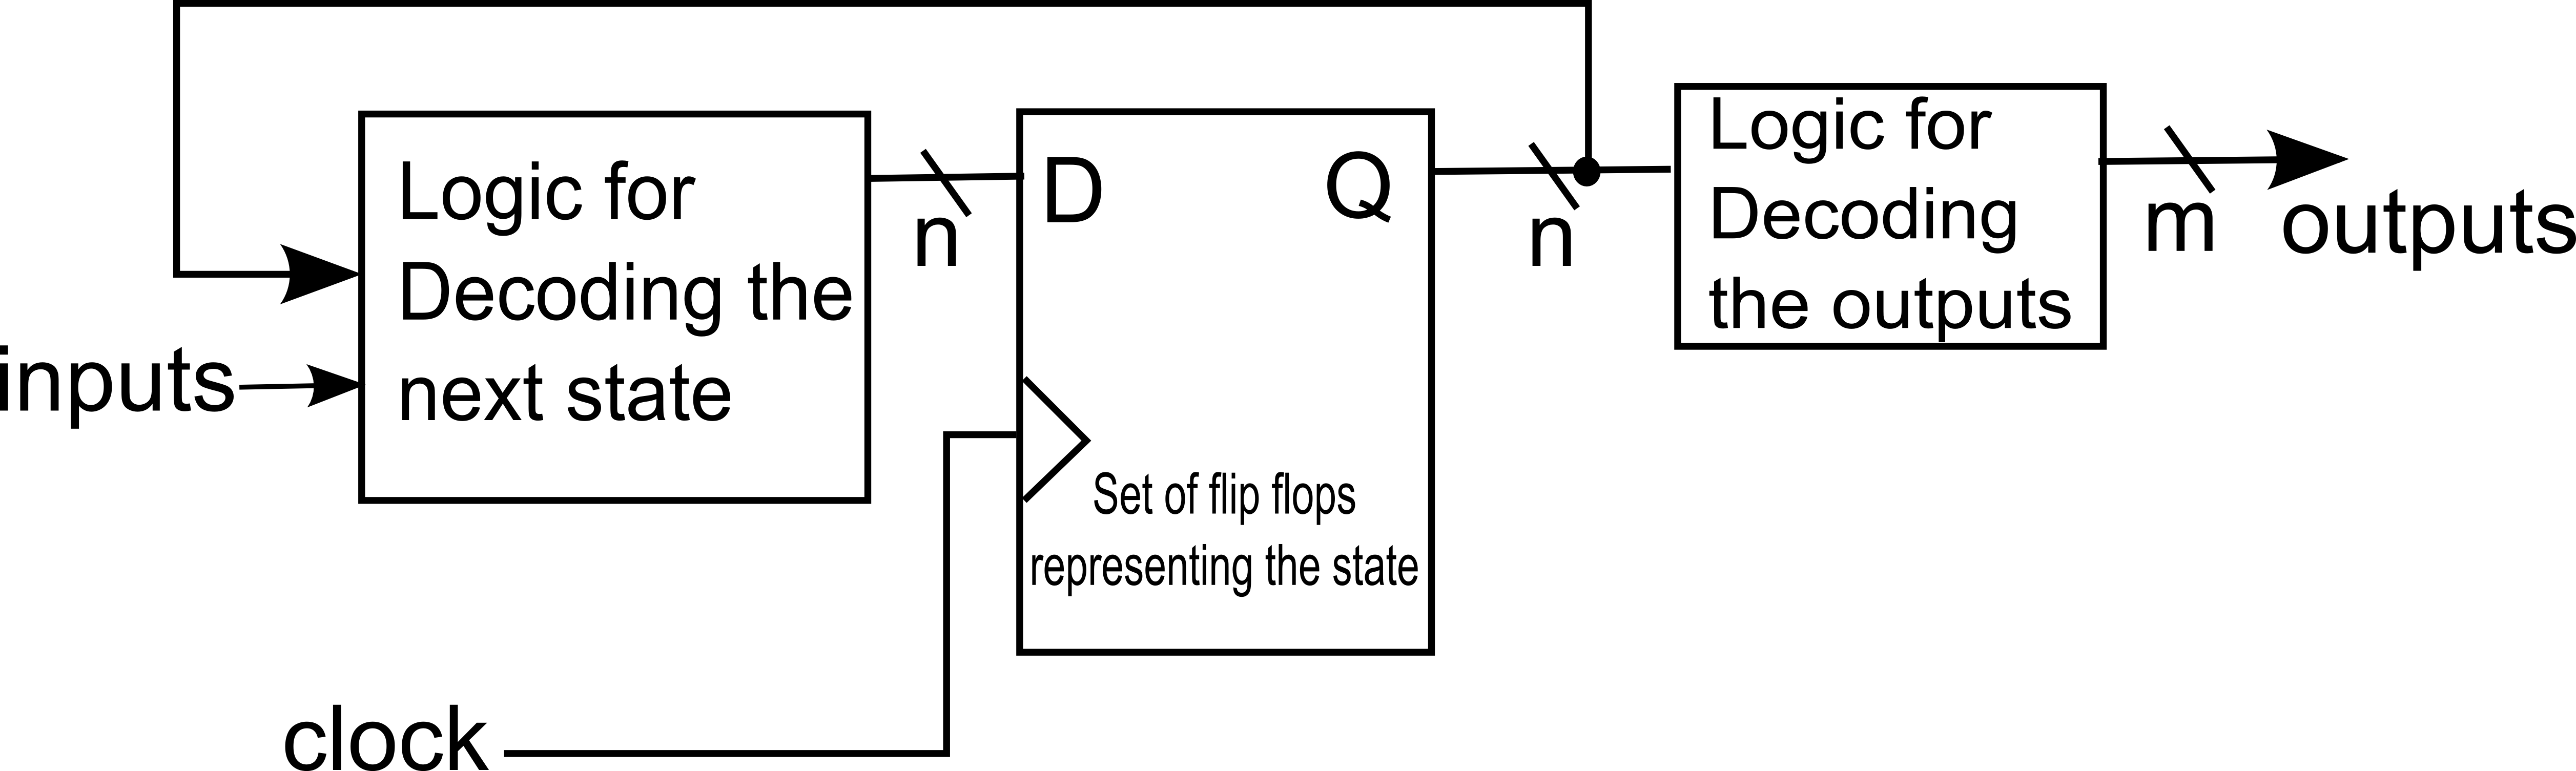
\includegraphics[width=.7\textwidth]{fsm}
  \caption{Basic finite state machine block diagram (Figure from \cite{fsm})}
  \label{fig:fsm}
\end{figure}

The justification for the aim to create a device which can emulate any 10-input, 10-output,
10-state FSM is the hope that such a specific goal will help to ground the abstract
nature of FPGA's. With this goal in mind, design decisions 'tiebreakers' can be
handled more easily because the answer to the difficult question of deciding on important
variables is always "Which value will give better results to the goal FSM circut?".
The basic setup of this FSM type design can be seen in Figure \ref{fig:fsm} above.

\newpage
\section{Circuit Design}

\subsection{Architecture}

\begin{figure}[htb]
  \centering
  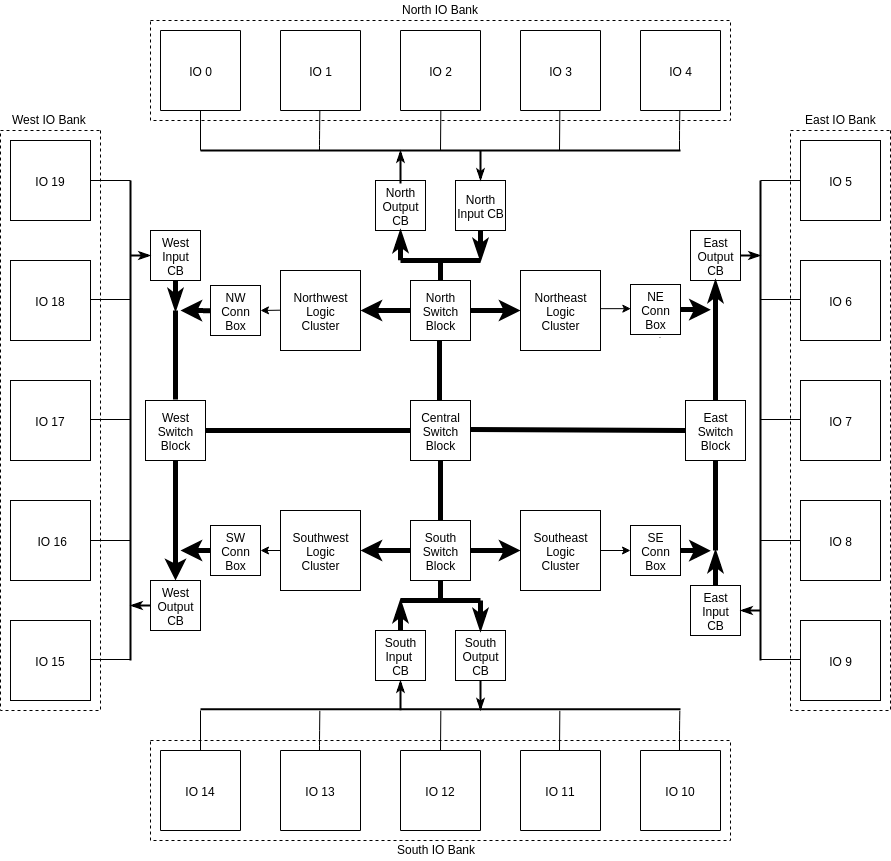
\includegraphics[width=.9\textwidth]{internal_block}
  \caption{Block diagram for new architecture}
  \label{fig:internal_block}
\end{figure}

The design of this architecture attempts to mimic the well established island FPGA 
architecture from Section \ref{Architecture} although it is too small to really draw parallels between the two.
The specific internal block diagram for this project can be seen in Figure \ref{fig:internal_block},
made up from 20 IO blocks, 5 switch blocks, 12 connection boxes, and 4 logic clusters.
The fabric of the FPGA is 10 wires wide represented
by the thicker lines connecting the switch blocks and connection boxes.

The general size of this architecture was decided based on the need for an architecture
which could be routed by hand if enough progress was not made on the place/route/bitstream software
tool set. This size is definitely limiting when attempting to implement general
verilog designs but is actually very helpful when working out and planning a configuration
for a gate-level diagram by hand which was done many times during the development process
to get a better understanding of how each block works together. In alignment with the overarching
goal for this circuit to implement the medium sized FSM, this design provides the correct amount
of IO's and provides more than 5 times the required amount of state storage. This gives much lenience 
to the HDL programmer to design state storage in less efficient (but more logical) ways and leaves
plenty of room to implement next state and output conversion logic (Figure \ref{fig:fsm}).

The design has 4 Banks of 5 IO blocks. The north and south blocks are biased towards inputs
as they can be routed to the input pins of a logic cluster by going through only a single switch
block. The east and west blocks are biased towards outputs as they can be routed to from a logic
cluster in one or less switch block connections. This decision attempts to remove the necessity 
of the use of global routing resources by allowing a number of signals
in well designed circuits to avoid going through the center switch block (where each signal can
consume a maximum of 10\% of the total global wires).

\subsection{Programming Circuit}

\begin{figure}[htb]
  \centering
  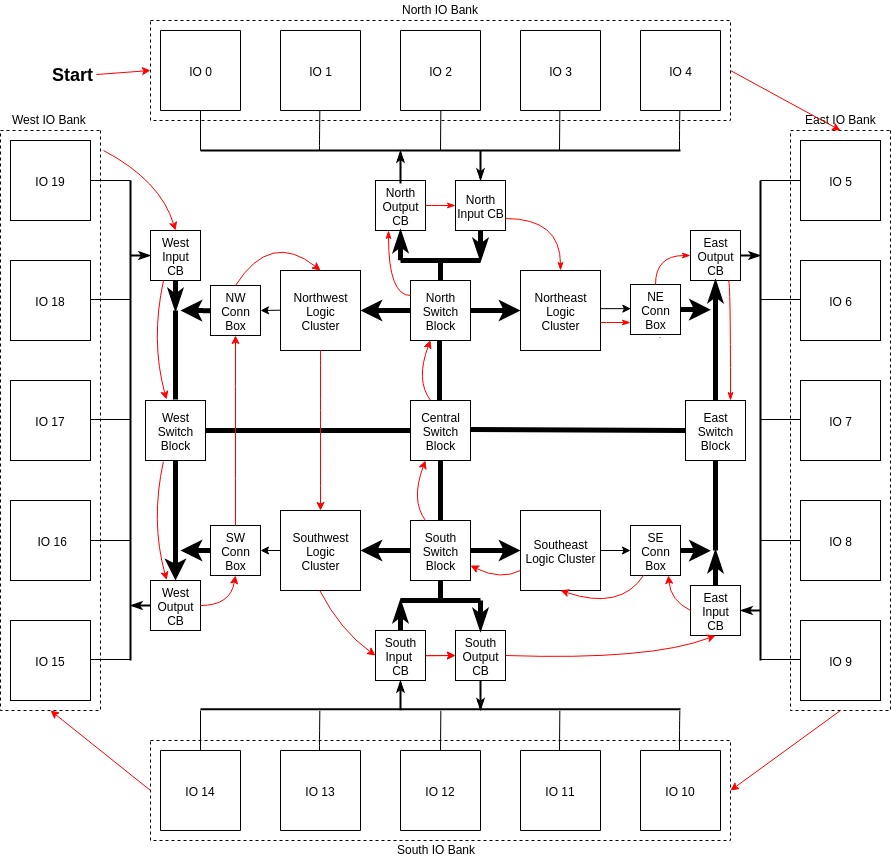
\includegraphics[width=.6\textwidth]{prog_diag}
  \caption{Block diagram for new architecture with programming order}
  \label{fig:prog_diag}
\end{figure}

As is required to achieve the design goals for this circuit, all of the settings for
each block are completely configurable through a ‘snake’ of shift registers that runs throughout 
the circuit (Figure \ref{fig:prog_diag}). The programming order chosen was based on connecting
spatially close blocks. Originally, this was done with only clock and data
wires. An additional enable wire was added to both decrease the probability of the circuit
being changed by noise during use, and to more easily internally detect when the
in-circuit programming was complete.

\subsection{Basic Logic Element}

\begin{figure}[ht]
    \centering
    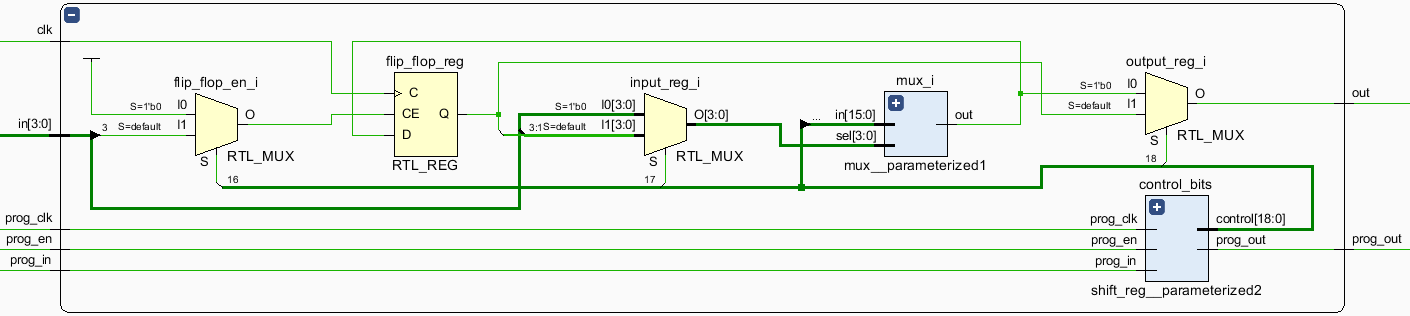
\includegraphics[width=\textwidth]{ble}
    \caption{Basic logic element circuit diagram}
    \label{fig:ble}
\end{figure}

The design of the BLE block is very basic. The block design can be seen in Figure 
\ref{fig:ble} and the verilog code can be found in the code listing section of the
appendix (Figure \ref{code:ble}). The BLE contains 3 2-bit muxes,
1 16-bit mux, and 2 19 bit shift registers, 16 bits of which are used in the 4-
LUT. The remaining 3 bits are used to: enable the feedback path from the flip flop 
to input A of the 4-LUT, enable the use of input D as the enable input to the flip 
flop, and lastly to select the flip flop as output or the 4-LUT as the output. This 
design will aid in simplicity of circuit verification and in implementation routing.
The addition of two sets of shift registers was discovered to be required during 
simulation as the circuit would enter into invalid states while being programmed. 
To combat this problem, there are two banks of shift registers. The first is used 
only while the device is being programmed (as told by the prog{\_}enable signal). The 
second is only filled when the final control signals are in the programming shift 
registers (falling edge of prog{\_}enable signal).

\subsection{Connection Box}

\begin{figure}[ht]
    \centering
    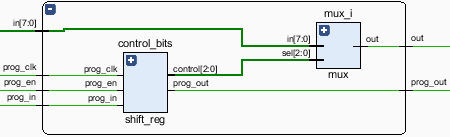
\includegraphics[width=\textwidth]{prog_mux}
    \caption{Circuit diagram of a programmable multiplexer}
    \label{fig:prog_mux}
\end{figure}

The connection box implementation is based on the combination of many less complicated
logic blocks called programmable multiplexers (prog mux). A prog mux is simply a mux combined with
a shift register which is in the configuration chain of the FPGA. This enables the logic
block to be connected to a number of inputs in hardware but have the ultimate selection
of which wire to drive to the output done at programming time as part of the bitstream. 
A graphical representation of this block can be seen in Figure \ref{fig:prog_mux}.

Once the prog mux block is created, the design for a connection box is relatively simple
as described in Section \ref{Conn_Box}. A prog mux is created for each output pin. The
size (number of select bits) of the prog mux is determined by taking the ceiling of
the log base 2 of the number of inputs.
The use of Verilog parameters (as seen in Figure \ref{code:prog_mux} and Figure \ref{code:conn_box})
makes both the connection box and the prog mux reusable
throughout the rest of the HDL design.

\subsection{Logic Cluster}

\begin{figure}[ht]
    \centering
    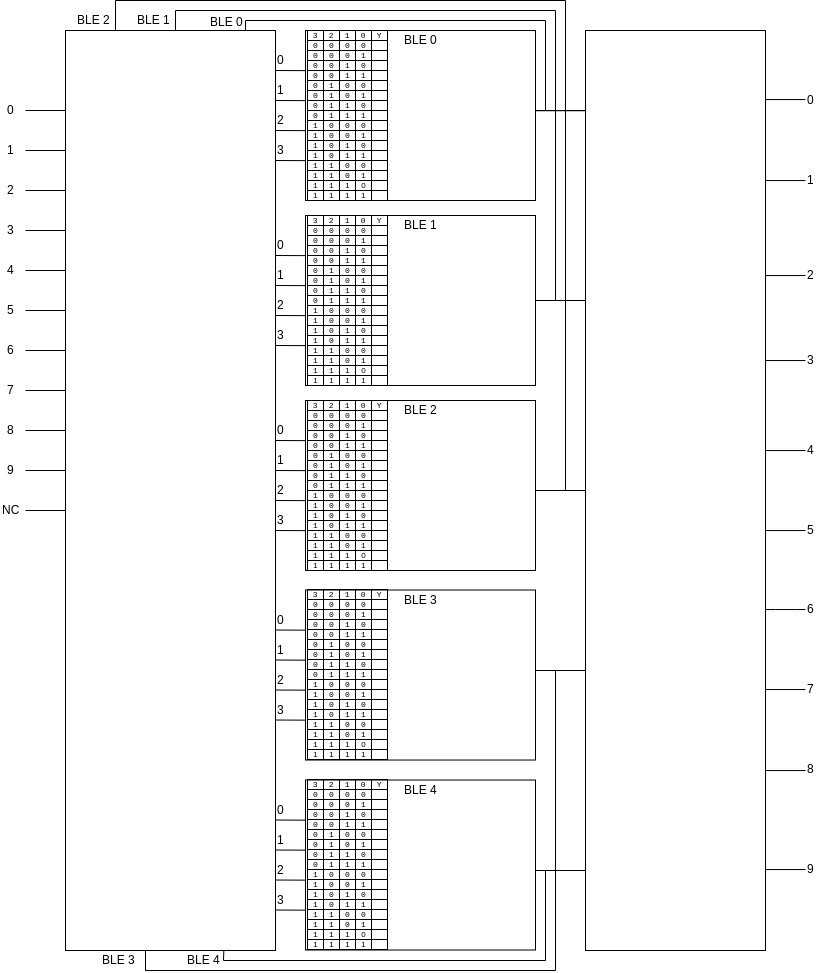
\includegraphics[width=0.5\textwidth]{LogicCluster}
    \caption{Logic cluster diagram (including output connection box)}
    \label{fig:logic_cluster}
\end{figure}

The logic cluster is a combination of a connection box and multiple basic logic elements
as discussed in Section \ref{logicCluster}. The number of ble's was chosen to be 5. This
was a value that seemed reasonable in regards to how much total memory and logic resources
 it produced. It also allowed the use of 16 input prog muxes (instead of 32 input) with a
10 bit fabric bus. The choice of 6 ble's also would have allowed the use of 16 input prog muxes but
5 ble's times 4 logic clusters already provided more than enough resources to achieve the
FSM goal.

The graphic in Figure \ref{fig:logic_cluster} is a good way to represent the entire view
of a logic cluster. This diagram was printed out and used to walk though the place and route problem in
complete detail. Lines can be drawn in both connection boxes to show connections to and from ble's while
gate level diagrams can be drawn in each ble block and then translated into the look up table
equivalent. This process was done many times during development to ensure understanding of
how everything fit together.

\subsection{Switch Block}

The switch block design uses the disjoint connection pattern to create the simplest
possible fabric structure. The block has 4 10 bit wide bus connections which are all
bidirectional. The internal makeup of the switch block is (like the connection box) just
made up of many prog muxes driving the output pins of each pin of the bus connections with
an additional connection for not driving the output (High Z).


\subsection{Input/Output Block}

The IO block was influenced by the complicated Xilinx model referenced in Figure
\ref{fig:complex_io} but reduced significantly. It consists of the minimum setup 
(a few tri-state drivers) plus pull up/down resistors with pass transistor 
enables, and the shift registers required to program it. The pull-up and pull-down
resistors however, are not applicable when dealing with this Verilog implementation
and static digital simulation.

\newpage
\section{Verilog-to-Routing}

\subsection{Introduction}

Verilog-to-Routing (VTR) \cite{vtr} is the premiere open source FPGA CAD flow for FPGA academic research.
This tool allows any FPGA architecture to be worked on with the use of its architecture
description language to specify every detail about the architecture.
The fact that this tool was discovered aided the project tremendously due to how many
complex algorithms could be left to VTR to handle. VTR is comprised of 3 separate tools:
Odin, ABC, and VPR. Odin is used to synthesize and elaborate Verilog files into 
BLIF netlist files which can be
implemented on the specified architecture. The next tool executed is ABC which optimizes the
netlist. Versatile Place and Route (VPR) is the final step in the flow which takes the
netlist produced in the previous step and places the individual groups of logic 
and routes the nets on the architecture. VPR also provides a graphical representation to view
how the circuit is implemented on the device.

While the original goal of this project was to create an FPGA from scratch (including
the software tools) the use of VTR was deemed to be a good decision for two main reasons.
First, VTR is a sort of academic standard and provides all sorts of additional
features (not used in this project) to help benchmark and compare FPGA architectures.
Therefore, this was seen as a good opportunity to learn a new toolset in a hands on manor for
possible future projects in this area of study. Second, The algorithms that VTR handles
are REALLY complex (NP-Hard) and also creates the opportunity
to implement Verilog designs instead of hand produced netlists and logic. Specifically the VPR tool
provides a way to avoid writing a new place and route algorithm which would have
been passable with this size of architecture but would have struggled with any increase
in size (as a good place and route algorithm could be a whole senior project on its own).

\subsection{Architecture Description}

\begin{figure}[H]
    \centering
    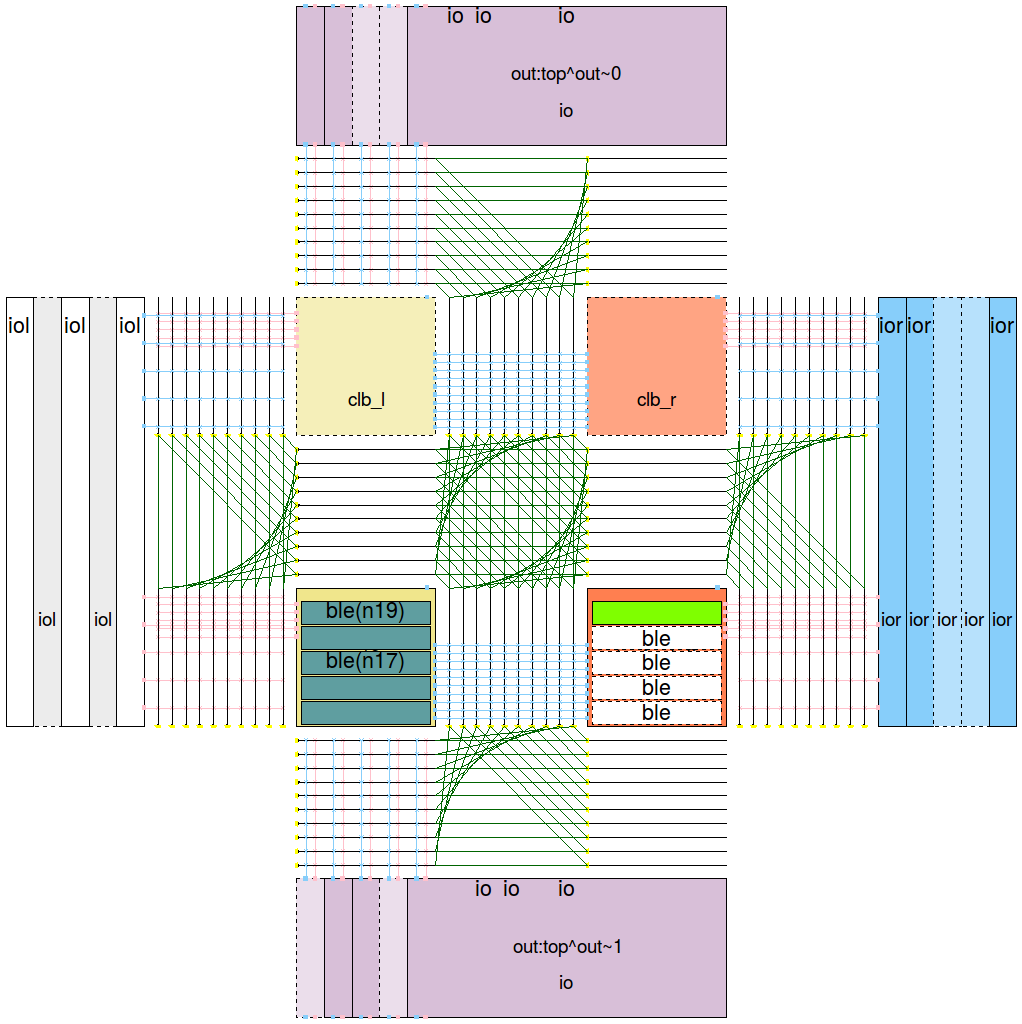
\includegraphics[width=0.75\textwidth]{vtr_arch}
    \caption{VTR parse and rendering of new architecture}
    \label{fig:vtr_arch}
\end{figure}

In order to integrate with the VTR CAD flow both a Verilog file and an architecture
description file must be
provided. The Verilog is easy and marks a huge improvement over hand drawing circuits
and feeding them into a hand-written tool, but the architecture description language
is a whole other concept to grasp. This language uses an XML format to specify every
possible variable within an architecture including: setup-hold times, switch block
connection strategy, block locations, BLE size, and much more. For this project, all
timing information was deemed to be out of scope so there are placeholder times, resistances,
and capacitances where real values should be (VTR did not accept the concept of
an 'ideal' FPGA and refused to route it). This commented file can be found in the Appendix
in Listing \ref{code:arch_des}
and it produces the graphical representation found in Figure \ref{fig:vtr_arch}.

As can be seen in Figure \ref{fig:vtr_arch}, there are slight differences in how VTR
perceives this architecture vs how it was designed (Figure \ref{fig:internal_block}).
These differences are mainly present in the fabric and switch block layout and are
due to the lack of granularity control in specifying the location of the fabric and switch blocks.
The VTR tool makes the assumption that the architecture being specified is a regular
island type architecture (which has a very regular fabric structure) and spends much
more effort in understanding the various complex blocks (IO, logic cluster, BLE, etc).
This difference is entirely cosmetic as there is still a strict equivilance between
the channels from the designed to the interpreted architectures which is important for
generating the bitstream.

Another notable diversion from the design specified is that many of the auxiliary control 
signals for the BLE implementation are missing from the architecture specification file
(internal feedback and flip flop enable) due to being able specify them in the architecture file.
These features are still in the HDL implementation of the device and still accessible via hand
programming although they will be unknown (and unusable) to the VTR flow.

\subsection{Example}

The main example that will be used in this report is a simple sequence detector circuit
with an output bus that drives a seven-segment display with the current state. This is
a classic example of a FSM type of design although it only has 3 inputs (including clock)
and 7 outputs. The design recognizes the 9-bit long sequence "101100101" which takes
9 states (one for each bit of the sequence) and one additional state for an initial zero.
This can be seen in more detail in the code listing for this example (Listing \ref{code:seq_det}).
Figure \ref{fig:seq_det} showcases this example circuit implemented on the new architecture.
Some notable observations include how the concept of input and output biased IO banks
are not taken into account. Also it is surprising to see 100\% BLE utilization
within the architecture with this design. Usually, routing resources are the main
obstacle in the implementation onto an FPGA. Anywhere from 85\%-90\% logic utilization
is usually where commercial place and route algorithms begin to struggle to successfully
route designs.

\begin{figure}[H]
    \centering
    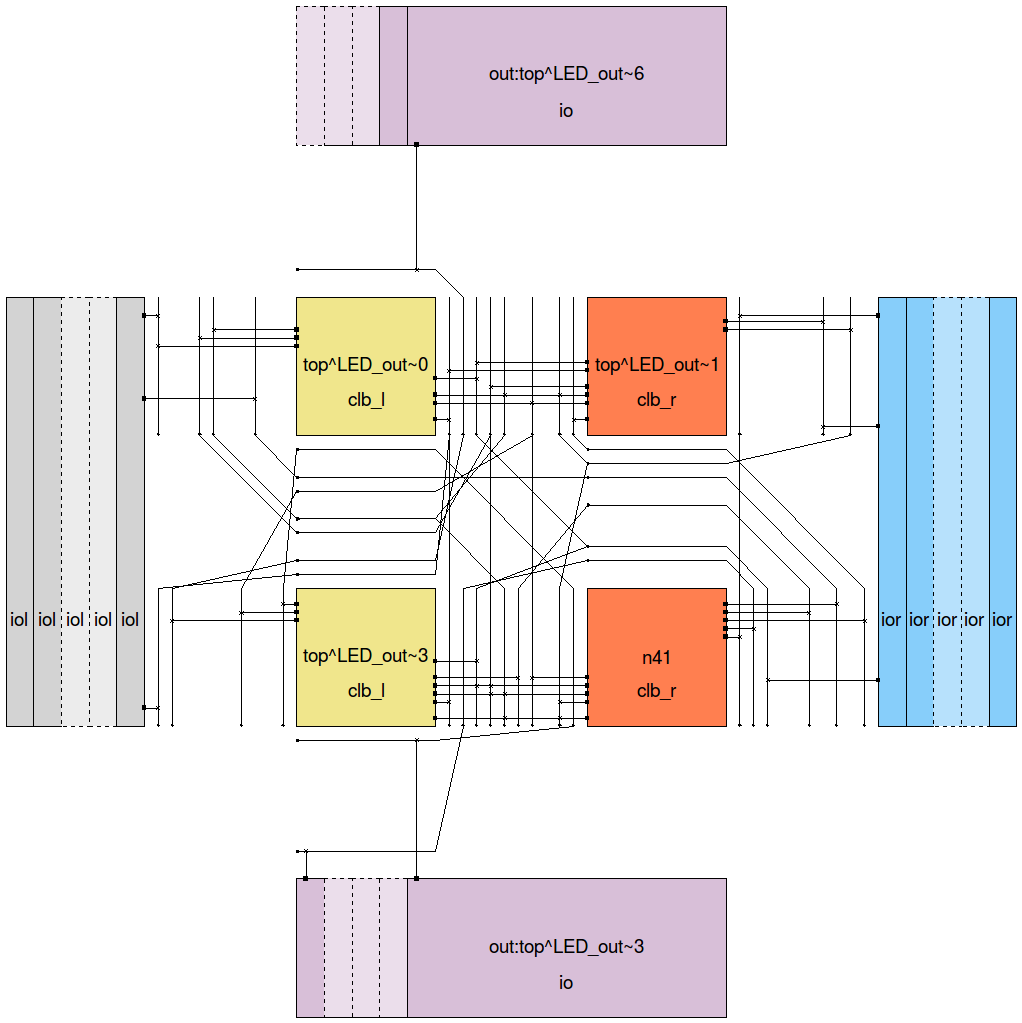
\includegraphics[width=0.9\textwidth]{seq_det}
    \caption{VTR rendering of sequence detector implementation}
    \label{fig:seq_det}
\end{figure}

\newpage
\section{Bitstream Generation}

\subsection{VTR File Parsing}

\subsection{Design}

\newpage
\section{Circuit Verification}

\subsection{Basic Logic Element}

\subsection{Connection Box}

\subsection{Logic Cluster}

\subsection{Switch Block}

\subsection{Input/Output Block}

\newpage
\section{Conclusion}

\newpage
\bibliography{fpga_report}{}
\addcontentsline{toc}{section}{References}
\bibliographystyle{plain}

\newpage
\section{Appendix}

\subsection{Github}

\subsection{Architecture Description File}

\lstinputlisting[language=xml,caption={Architecture description file}, label={code:arch_des}]{../vtr/basic.xml}

\subsection{Design Code Listing}

\lstinputlisting[language=Verilog, caption={Basic logic element code}, label={code:ble}]{../src/logic_element.v}

\subsection{Testbench Code Listing}


\subsection{Bitstream Generator Code Listing}


\end{document}
